%% LyX 2.3.6 created this file.  For more info, see http://www.lyx.org/.
%% Do not edit unless you really know what you are doing.
\documentclass[english,aspectratio=169]{beamer}
\usepackage{lmodern}
\renewcommand{\sfdefault}{lmss}
\renewcommand{\ttdefault}{lmtt}
\usepackage[T1]{fontenc}
\usepackage[latin9]{inputenc}
\setlength{\parskip}{\medskipamount}
\setlength{\parindent}{0pt}
\usepackage{babel}
\usepackage{url}
\usepackage{amssymb}
\usepackage{graphicx}
\PassOptionsToPackage{normalem}{ulem}
\usepackage{ulem}
\ifx\hypersetup\undefined
  \AtBeginDocument{%
    \hypersetup{unicode=true}
  }
\else
  \hypersetup{unicode=true}
\fi

\makeatletter

%%%%%%%%%%%%%%%%%%%%%%%%%%%%%% LyX specific LaTeX commands.
\pdfpageheight\paperheight
\pdfpagewidth\paperwidth

%% A simple dot to overcome graphicx limitations
\newcommand{\lyxdot}{.}


%%%%%%%%%%%%%%%%%%%%%%%%%%%%%% Textclass specific LaTeX commands.
% this default might be overridden by plain title style
\newcommand\makebeamertitle{\frame{\maketitle}}%
% (ERT) argument for the TOC
\AtBeginDocument{%
  \let\origtableofcontents=\tableofcontents
  \def\tableofcontents{\@ifnextchar[{\origtableofcontents}{\gobbletableofcontents}}
  \def\gobbletableofcontents#1{\origtableofcontents}
}

%%%%%%%%%%%%%%%%%%%%%%%%%%%%%% User specified LaTeX commands.
\usetheme{CambridgeUS}
%\usecolortheme{dove}
\hypersetup{pdfpagemode=None}
\usepackage{tikz}
\usepackage{color}
\usepackage{listings}

% This allows to change color of symbols in math
\newcommand*{\mathcolor}{}
\def\mathcolor#1#{\mathcoloraux{#1}}
\newcommand*{\mathcoloraux}[3]{%
  \protect\leavevmode
  \begingroup
    \color#1{#2}#3%
  \endgroup
}

\makeatother

\begin{document}
\title[Theory ]{Scientific Computing and Data Management}
\author{Marcello Vichi}
\institute[UCT]{Department of Oceanography\\marcello.vichi@uct.ac.za}
\date{Applied Ocean Sciences}
\makebeamertitle

\section*{Outlines}
\begin{frame}{Outline}

\tableofcontents{}
\end{frame}

\section{Scientific Computing and Data Management}
\begin{frame}{Oceanography is an observational and computational science}

\begin{fact}
Ocean scientists collect data or access data collected by others
\end{fact}

\begin{itemize}
\item {\small{}Many scientists choose to work with a specific software for
data analysis and visualization but soon realize that much of the
work is not only writing computationally intensive number-crunching
loops}{\small\par}
\item {\small{}Very often programming is about }\textbf{\small{}shuffling
data in and out of different tools, converting one data format to
another, extracting numerical data from a text, and administering
experiments involving a large number of data files and directories}{\small{}.
(HP Langtangen, Python Scripting for Computational Science, 2008)}{\small\par}
\item This workflow must be properly organized, no matter which operating
system or software you have chosen
\end{itemize}
\end{frame}
%
\begin{frame}{The data<->science workflow}

The aim of this course is to increase the productivity of your data-to-science
workflow, by presenting you with a few examples of methodologies and
tools
\begin{enumerate}
\item Production/Collection \emph{(Investigation and Meta-search)}
\item Retrieval \emph{(Transfer)}
\item Data Management \emph{(Short-term archival and meta-data)}
\item Processing \emph{(Programming and Revision control)}
\item Analysis \emph{(Programming and Revision control)}
\item Publication or Higher Level Production \emph{(Programming, Revision
control and meta-data)}
\item Data Management \emph{(Long-term archival and meta-data)}
\end{enumerate}
\end{frame}
%
\begin{frame}{Data Management (DM)}

\framesubtitle{Adapted from the lecture notes by R. Roman and D. Byrne}

Data management comprises the following items:
\begin{itemize}
\item data collection
\item organisation
\item storage
\item preservation
\item publication
\end{itemize}
\end{frame}
%
\begin{frame}{Why do we need DM?}
\begin{itemize}
\item Government and research data, collected at public expense, must be
properly managed in order to realize their full potential and justify
their considerable production and maintenance costs
\item Your institution's and funding agency's expectations and policies
\item To ensure research integrity and validation of results.
\item To increase research efficiency
\item To facilitate data security and minimise the risk of data loss
\item To ensure wider dissemination and increased impact
\item To enable research continuity through secondary data use (permit new
and innovative research to be built on existing information)
\item Uniqueness of observations => you can\textquoteright t measure a 2001
temperature next year!
\item Journals now request data to be made available on line for the study
to be validated (Retraction watch) \href{https://retractionwatch.com/}{https://retractionwatch.com/} 
\end{itemize}
\end{frame}
%
\begin{frame}{Preventing data loss}
\begin{columns}[t]

\column{6cm}
\begin{itemize}
\item - human error
\item - natural disaster
\item - facilities infrastructure failure
\item - storage failure
\item - server hardware/software failure
\item - application software failure
\end{itemize}

\column{6cm}
\begin{itemize}
\item - format obsolescence {[}floppy and stiffy drives{]}
\item - legal encumbrance
\item - malicious attack
\item - loss of staffing competencies
\item - loss of institutional commitment
\item - loss of financial stability
\end{itemize}
\end{columns}

\end{frame}
%
\begin{frame}{Principles of good DM}
\begin{itemize}
\item Define a research data management policy (University of Cape Town
data policy: \href{http://www.digitalservices.lib.uct.ac.za/dls/rdm-policy}{http://www.digitalservices.lib.uct.ac.za/dls/rdm-policy})
\item Data ownership (clear identification who has managerial and financial
control; legal rights along with copyright and intellectual property
rights)
\item Data documentation and metadata compilation {[}metadata applicable
to your field{]}
\item Data quality and standardisation
\item Data life-cycle control
\item Data custodian (not a person)
\item Data access and dissemination
\end{itemize}
\end{frame}
%
\begin{frame}{Definition: Research Data}

Research data is defined as \textbf{recorded factual material} commonly
retained by and accepted in the scientific community as necessary
to validate research findings \href{http://www.epsrc.ac.uk/about/standards/researchdata/scope}{http://www.epsrc.ac.uk/about/standards/researchdata/scope} 

Forms of research data
\begin{enumerate}
\item Observational (data captured in real-time. For example, sensor data,
survey data, sample data)
\item Experimental (data from lab equipment, often reproducible)
\item Simulations (data generated from models. For example climate and oceanic
models)
\item Derived/compiled (data is reproducible, text and data mining)
\item Reference (collection of peer-reviewed datasets that is published
and curated)
\end{enumerate}
\end{frame}
%
\begin{frame}{Data Management Plans}
\begin{columns}[t]

\column{6cm}

Most of the collected data in Ocean Sciences will ultimately become
\textbf{digital data}.

A DMP is always needed and considerations must be done prior to collecting
any data. 
\begin{itemize}
\item Types of data
\item Data sharing, access \& security, 
\item Metadata standards, 
\item re-use, archiving \& long-term preservation. 
\end{itemize}
Research data life cycle (Digital Curation Centre, \href{https://www.dcc.ac.uk}{www.dcc.ac.uk})

\column{6cm}

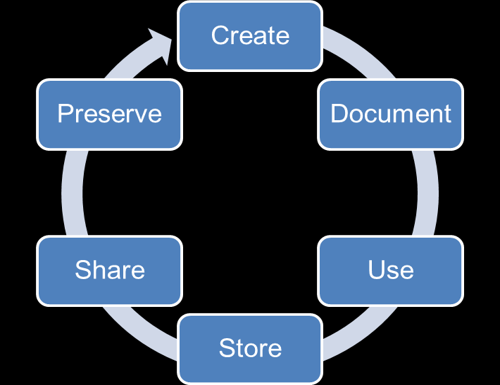
\includegraphics[width=6cm]{figures/DMP}
\end{columns}

\end{frame}
%

\begin{frame}{Data curation and visualization are recognized scholarly roles }
\begin{columns}[t]
\column{6cm}
\begin{itemize}
    \item Visualization - Preparation, creation and/or presentation of the published work, specifically visualization/data presentation.
    \item Data curation - Management activities to annotate (produce metadata), scrub data and maintain research data (including software code, where it is necessary for interpreting the data itself) for initial use and later re-use.
\end{itemize}
\column{6cm}

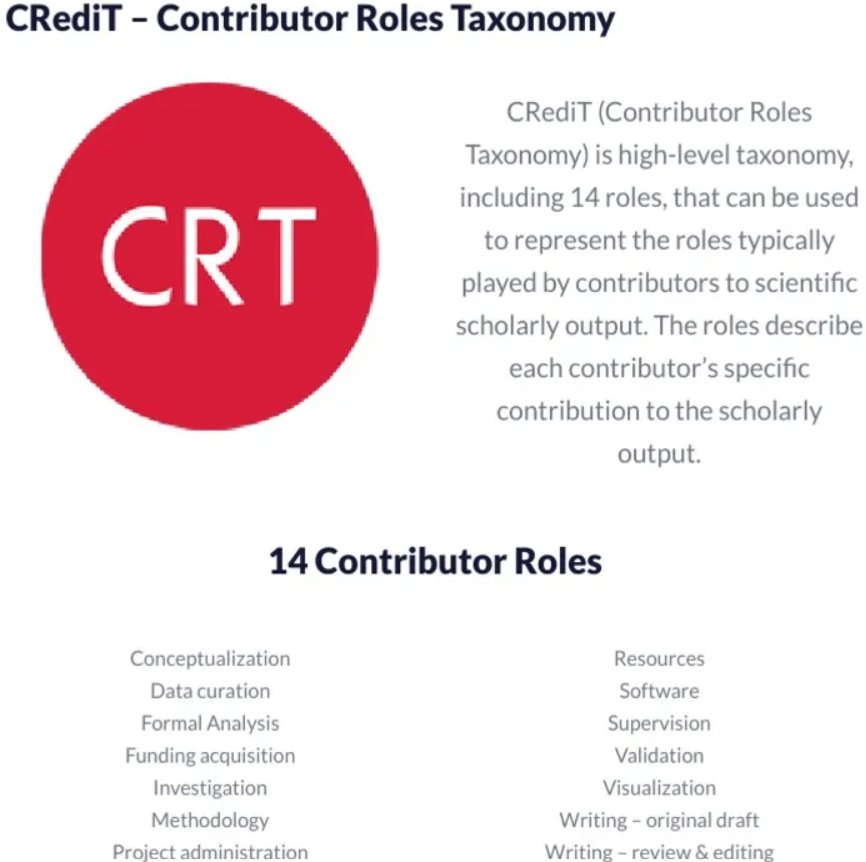
\includegraphics[width=6cm]{figures/credit.png}
\end{columns}

\end{frame}
%

\section{Digital data}
\begin{frame}{The computer interface}
\begin{itemize}
\item The ``computer'' is a logical processing unit that must be instructed
to perform operations (programmed)
\item It deals with information in a \textbf{digital} format, using electrical
signals that are temporarily stored in a physical space called memory
\item The ``inventors'' of the computer \emph{idea} (Turing and von Neumann)
created the mathematical methods to perform operations (program) and
to solve an \emph{infinite} set of problems. This developed the concept
of the \textbf{Central Processing Unit} of programmable computers 
\item This was the first giant leap: what was needed was creating the technical
possibility to do things according to this theoretical model. Translating
the operations in a machine language and returning the results in
a human-understandable language. The first working programmable computer
was done by Konrad Zuse in 1941. 
\item How do we interface with a computer?
\end{itemize}
\end{frame}
%
\begin{frame}{The operating system (OS)}

\begin{columns}[t]


\column{5cm}
\begin{itemize}
\item {\footnotesize{}The operating system is the agent that allows the
interaction between hardware (the components), software (the programs)
and the user \url{http://faculty.salina.k-state.edu/tim/ossg/Introduction/OSrole.html}}{\footnotesize\par}
\end{itemize}

\column{8cm}

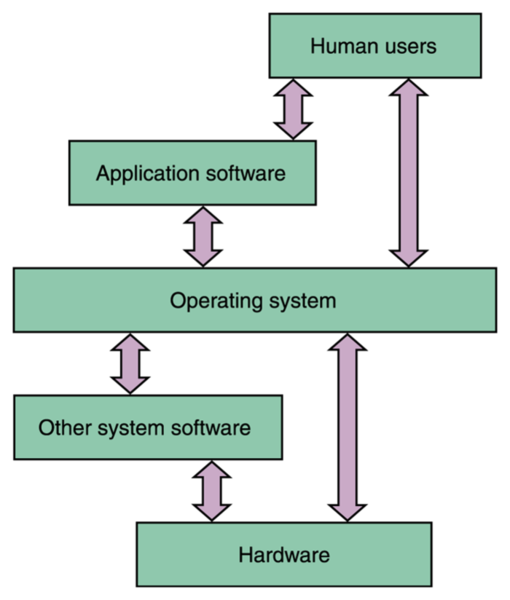
\includegraphics[width=6cm]{figures/OS_define}
\end{columns}

\end{frame}
%
\begin{frame}{What the OS does}

{\small{}The operating system is the }\textbf{\small{}software}{\small{}
}\textbf{\small{}interface}{\small{} that appears after the boot has
completed, and runs underneath all other programs - without it nothing
would happen at all. In simple terms, an operating system is a manager.
It manages all the available resources on a computer, from the CPU,
to memory, to network and hard disk accesses.}{\small\par}

{\small{}Tasks the operating system must perform:}{\small\par}
\begin{itemize}
\item {\small{}Control Hardware - The operating system controls all the
parts of the computer and attempts to get everything working together. }{\small\par}
\item {\small{}Run Applications - Another job the OS does is run application
software. This would include word processors, web browsers, games,
etc... }{\small\par}
\item {\small{}Manage Data and Files - The OS makes it easy for you to organize
your computer. Through the OS you are able to do a number of things
to data, including copy, move, delete, and rename it. This makes it
much easier to find and organize what you have}{\small\par}
\end{itemize}
\end{frame}
%
\begin{frame}{Types of OS}
\begin{itemize}
\item Windows (originally DOS)
\item Mac OSX (based on UNIX)
\item UNIX and Linux
\item Android and iOS
\item Virtual OS: host and guest (VirtualBox, VMware, etc)
\end{itemize}
\end{frame}
%
\begin{frame}{Giving instructions}

Operating systems have evolved considerably, from terminal prompts
to desktop managers. All modern OS allows you to give instructions
both through gestures (menu-click-drag-drop) and command line terminals

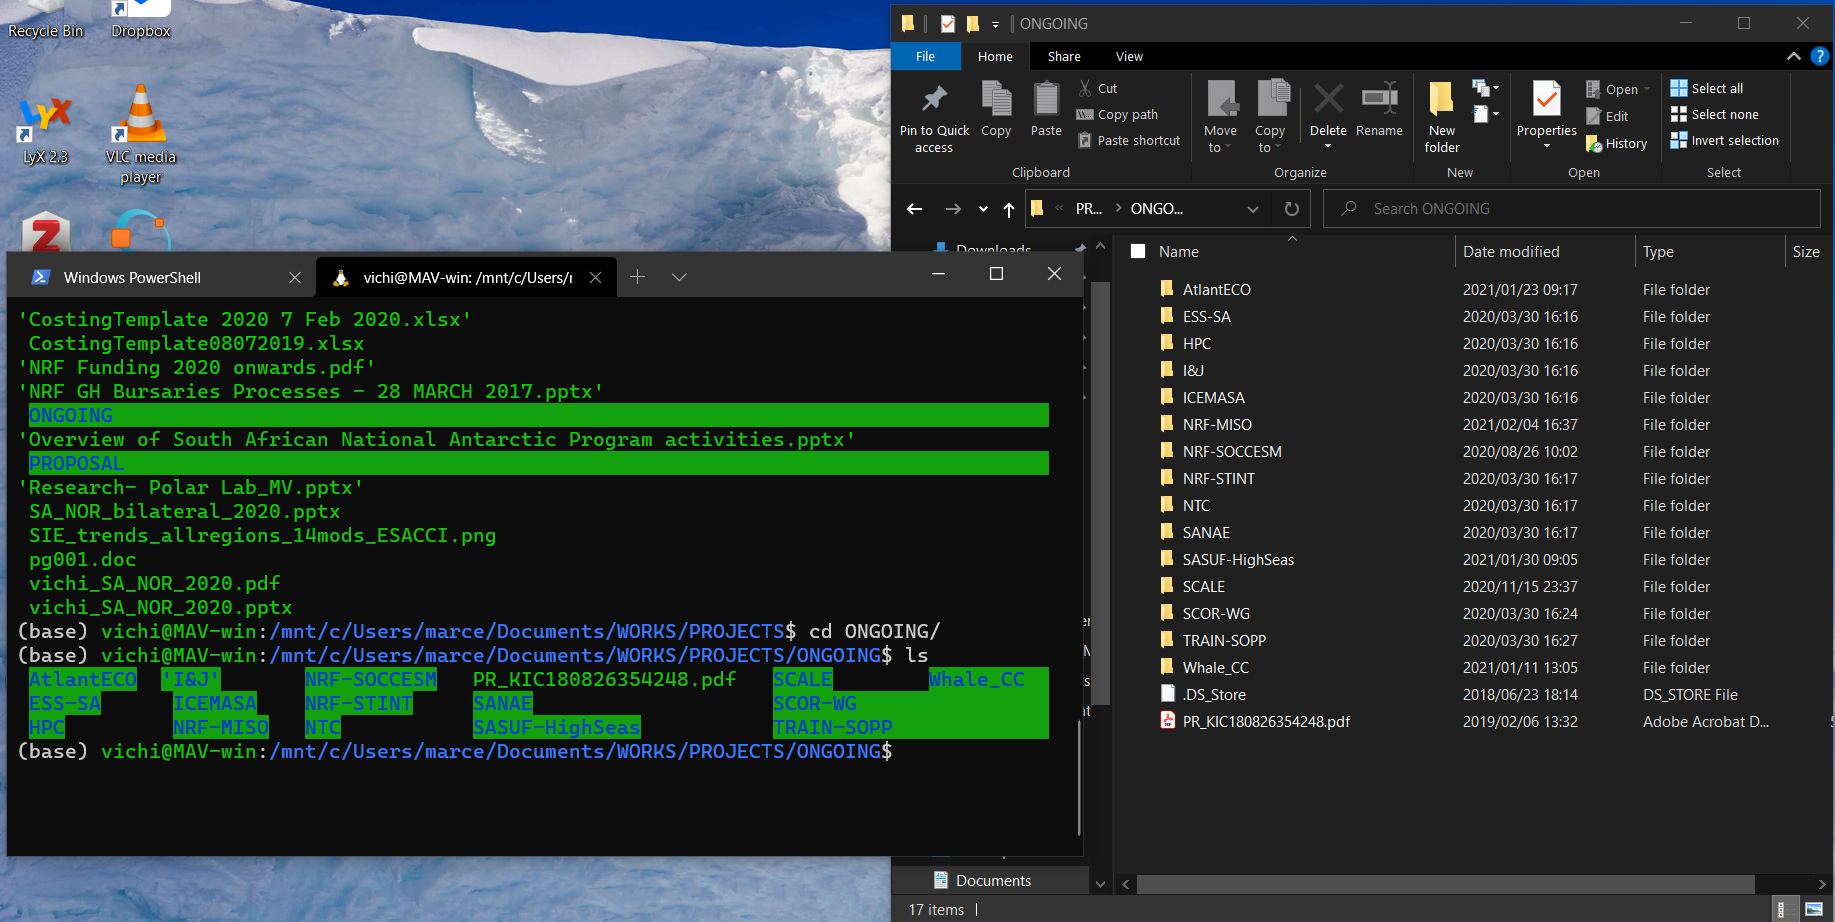
\includegraphics[scale=0.3]{figures/terminal_explorer}
\end{frame}
%
\begin{frame}{UNIX: a prototype for all OS}

The UNIX operating system was born in the late 1960s. It originally
began as a one-man project led by Ken Thompson of Bell Labs, and has
since grown to become the most widely used OS.
\begin{itemize}
\item In the time since UNIX was first developed, it has gone through many
different generations and even mutations.
\item Some differ substantially from the original version, like the Berkeley
Software Distribution (BSD, used on Mac OS) or Linux.
\item Other OSs still contain major portions that are based on the original
source code.
\item An interesting and rather up-to-date timeline of these variations
of UNIX can be found at \href{http://www.levenez.com/unix/history.html}{http://www.levenez.com/unix/history.html}
\end{itemize}
\end{frame}
%
\begin{frame}{Structure of the UNIX OS}
\begin{columns}[c]

\column{6cm}

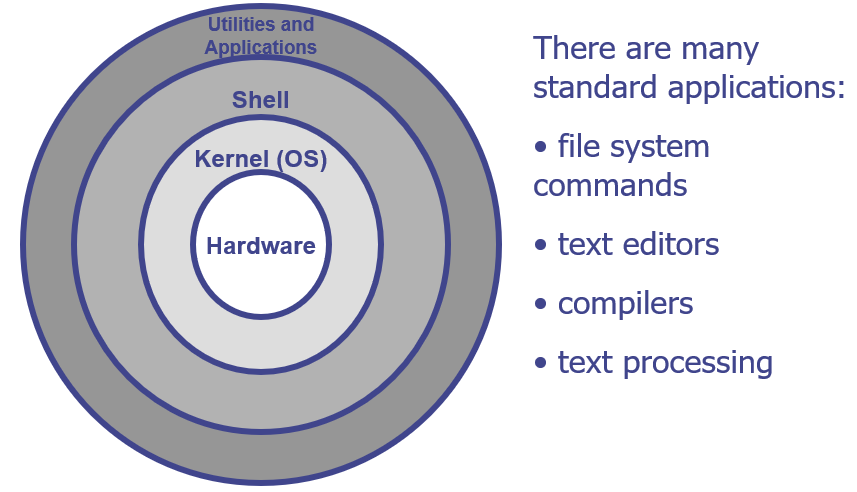
\includegraphics[width=6cm]{figures/unix_structure}
\begin{itemize}
\item {\scriptsize{}The Kernel - handles memory management, input and output
requests, and program scheduling. Technically speaking, the kernel
is the OS. It provides the basic software connection to the hardware.
The kernel is very complex and deals with the inner workings of these
things, and is beyond the scope of this course. }{\scriptsize\par}
\end{itemize}

\column{8cm}
\begin{itemize}
\item {\scriptsize{}The Shell and Graphical User Interfaces (GUIs) - the
}\emph{\scriptsize{}shell}{\scriptsize{} is a program that provides
a \textquotedblleft command line\textquotedblright{} interface where
the user can type commands. The GUI is similar, but commands are substituted
by graphical actions (buttons, menus, etc). These commands are translated
by the shell into something the kernel can comprehend, and then executed
by the kernel. }{\scriptsize\par}
\item {\scriptsize{}The Built-in System Utilities - are programs that allow
a user to perform tasks which involve complex actions. Utilities provide
user interface functions that are basic to an operating system, but
are too complex to be built into the shell. Examples of utilities
are programs that let us see the contents of a directory, move \&
copy files, remove files, etc... }{\scriptsize\par}
\item {\scriptsize{}Application Software \& Utilities -- these are not
part of the operating system. They are additional programs that are
bundled with the OS distribution, or available separately. These can
range from additional or different versions of basic utilities, to
full scale commercial applications}{\scriptsize\par}
\end{itemize}
\end{columns}

\end{frame}
%
\begin{frame}{Testing the command line}

\begin{itemize}
\item All operating systems have a command line interface. The commands
are typed by the user and executed using the enter key. To obtain
the list of files in a folder, test the following: 
\begin{itemize}
\item Windows app: \uline{Command prompt}. Launch the application and
type the command \texttt{dir}. 
\item Mac and Linux app: \uline{Terminal}. Launch the application and
type the command \texttt{ls}.
\end{itemize}
\item You will obtain the list of files in that folder. Some of them are
files of various types and some other are folders. Note that a folder
is also a file on the operating system: a file that contains a list
of other files
\end{itemize}
\end{frame}
%
\begin{frame}{Basic data types}
\begin{itemize}
\item {\small{}All machine-readable data are digital, which means that they
are made of coded }\textbf{\small{}discrete}{\small{} information}{\small\par}
\item {\small{}Data must have a format to be understood by the operating
system }{\small\par}
\begin{itemize}
\item \textbf{\small{}Binary data}{\small{}: contain the bits and bytes
of the information without a specific coding. They can be interpreted
by a software that knows already what to look for.}{\small\par}
\item \textbf{\small{}ASCII data}{\small{}: American Standard Code for Information
Interchange. An ASCII code is the numerical representation of a character,
which is still written in binary code but software know how to handle
the coding. 01101000 and 01101001 are equal to the decimal numbers
104 and 105, which in ASCII corresponds to the letters \textquotedbl hi\textquotedbl}{\small\par}
\end{itemize}
\item {\small{}A text produced with MS Word is a binary file, even if it
contains ASCII characters. This is because it includes formatting
information on how the document looks like. A text produced with a
}\emph{\small{}text editor}{\small{} (e.g. notepad) is instead an
ASCII file (often called a }\textbf{\small{}flat file}{\small{}).}{\small\par}
\item {\small{}A MS Excel ``table'' is not a flat file. Only if you save
it in ASCII format (e.g. using the Comma Separated Values format,
csv) it will be accessible by other ASCII applications.}{\small\par}
\end{itemize}
\end{frame}
%
\begin{frame}{Data transfer and protocols}
\begin{columns}[t]

\column{8cm}
\begin{itemize}
\item {\small{}Data must be on a support that is readable through a peripheral.
Nowadays we use files on }\emph{\small{}drives}{\small{} or through
the network. Originally (until the late 70's), the data were passed
through paper, the }\textbf{\small{}punch cards}{\small{}, then through
magnetic }\emph{\small{}floppy}{\small{} disks}{\small\par}
\item {\small{}On the Internet, data needs to be transferred in a coded
way. These methods are called protocols}{\small\par}
\begin{itemize}
\item \textbf{\small{}HTTP}{\small{}(S): hyper text transfer protocol (the
main protocol of browsers, written in HTML)}{\small\par}
\item \textbf{\small{}FTP}{\small{}: file transfer protocol (needs a terminal
or apps)}{\small\par}
\end{itemize}
\end{itemize}

\column{6cm}

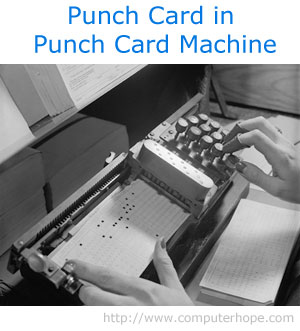
\includegraphics[width=4cm]{figures/punchcard}

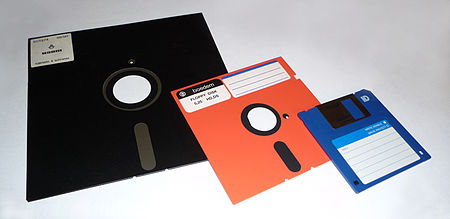
\includegraphics[width=6cm]{figures/450px-Floppy_disk_2009_G1}
\end{columns}

\end{frame}
%
\begin{frame}{Transfer and Storage: Apps or command line?}
\begin{columns}[t]

\column{4cm}
\begin{itemize}
\item {\tiny{}Data (file) transfer must be handled by specific applications
that know how to work with the protocols}{\tiny\par}
\item {\tiny{}This can be done through browsers, clients and command line
applications}{\tiny\par}
\item {\tiny{}Several public data archive allows to access their data via
several methods and for most of them it is possible to click on the
data we want}{\tiny\par}
\item {\tiny{}But what if we want more than one data file? We need to use
an application that allows this }\textbf{\tiny{}batch}{\tiny{} handling
or to write an ad hoc script executed through the command line }{\tiny\par}
\end{itemize}

\column{8cm}

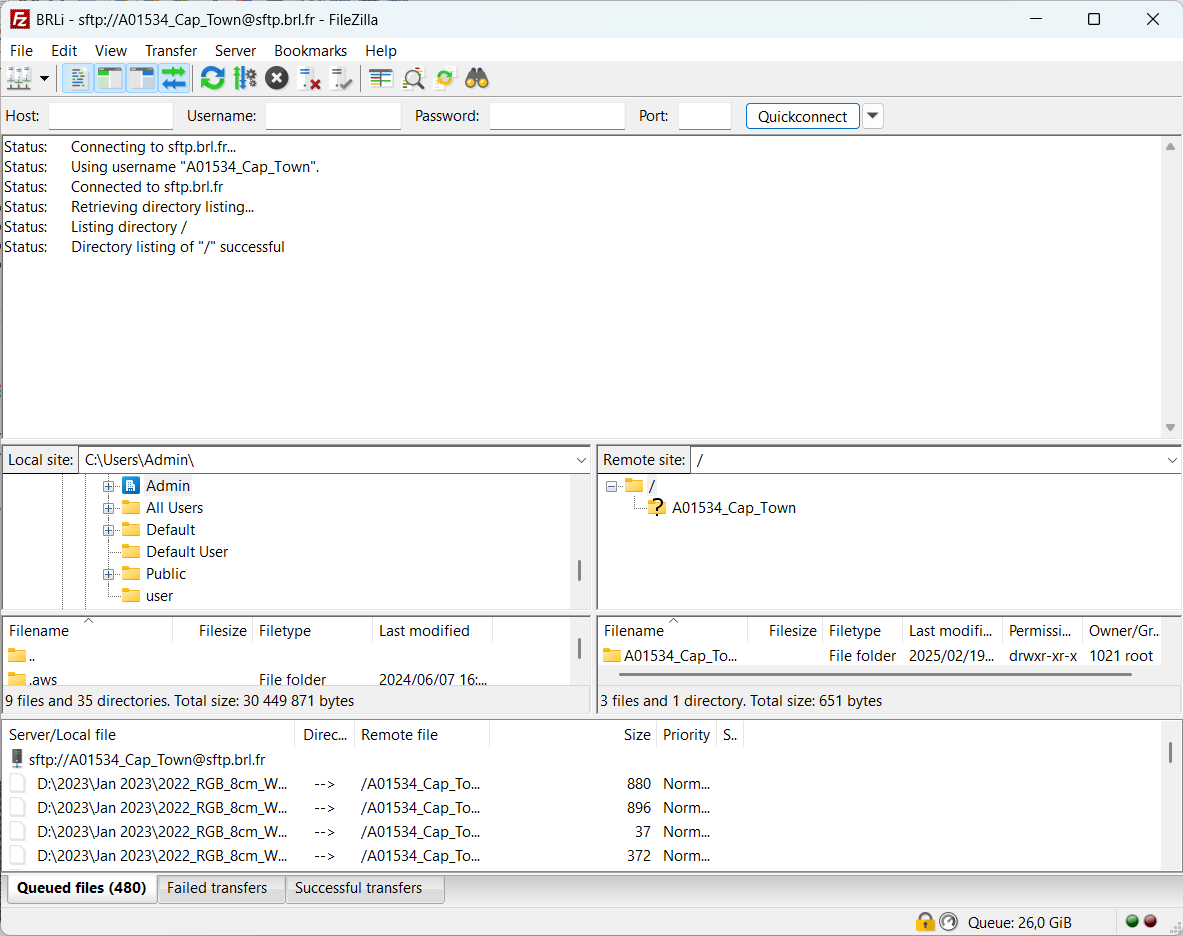
\includegraphics[width=3cm]{figures/ftp-browser}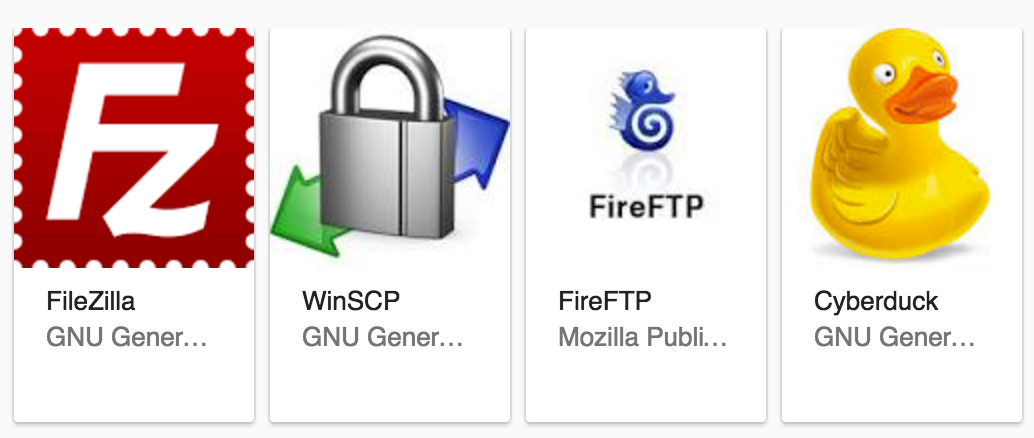
\includegraphics[width=4cm]{figures/ftp-clients}

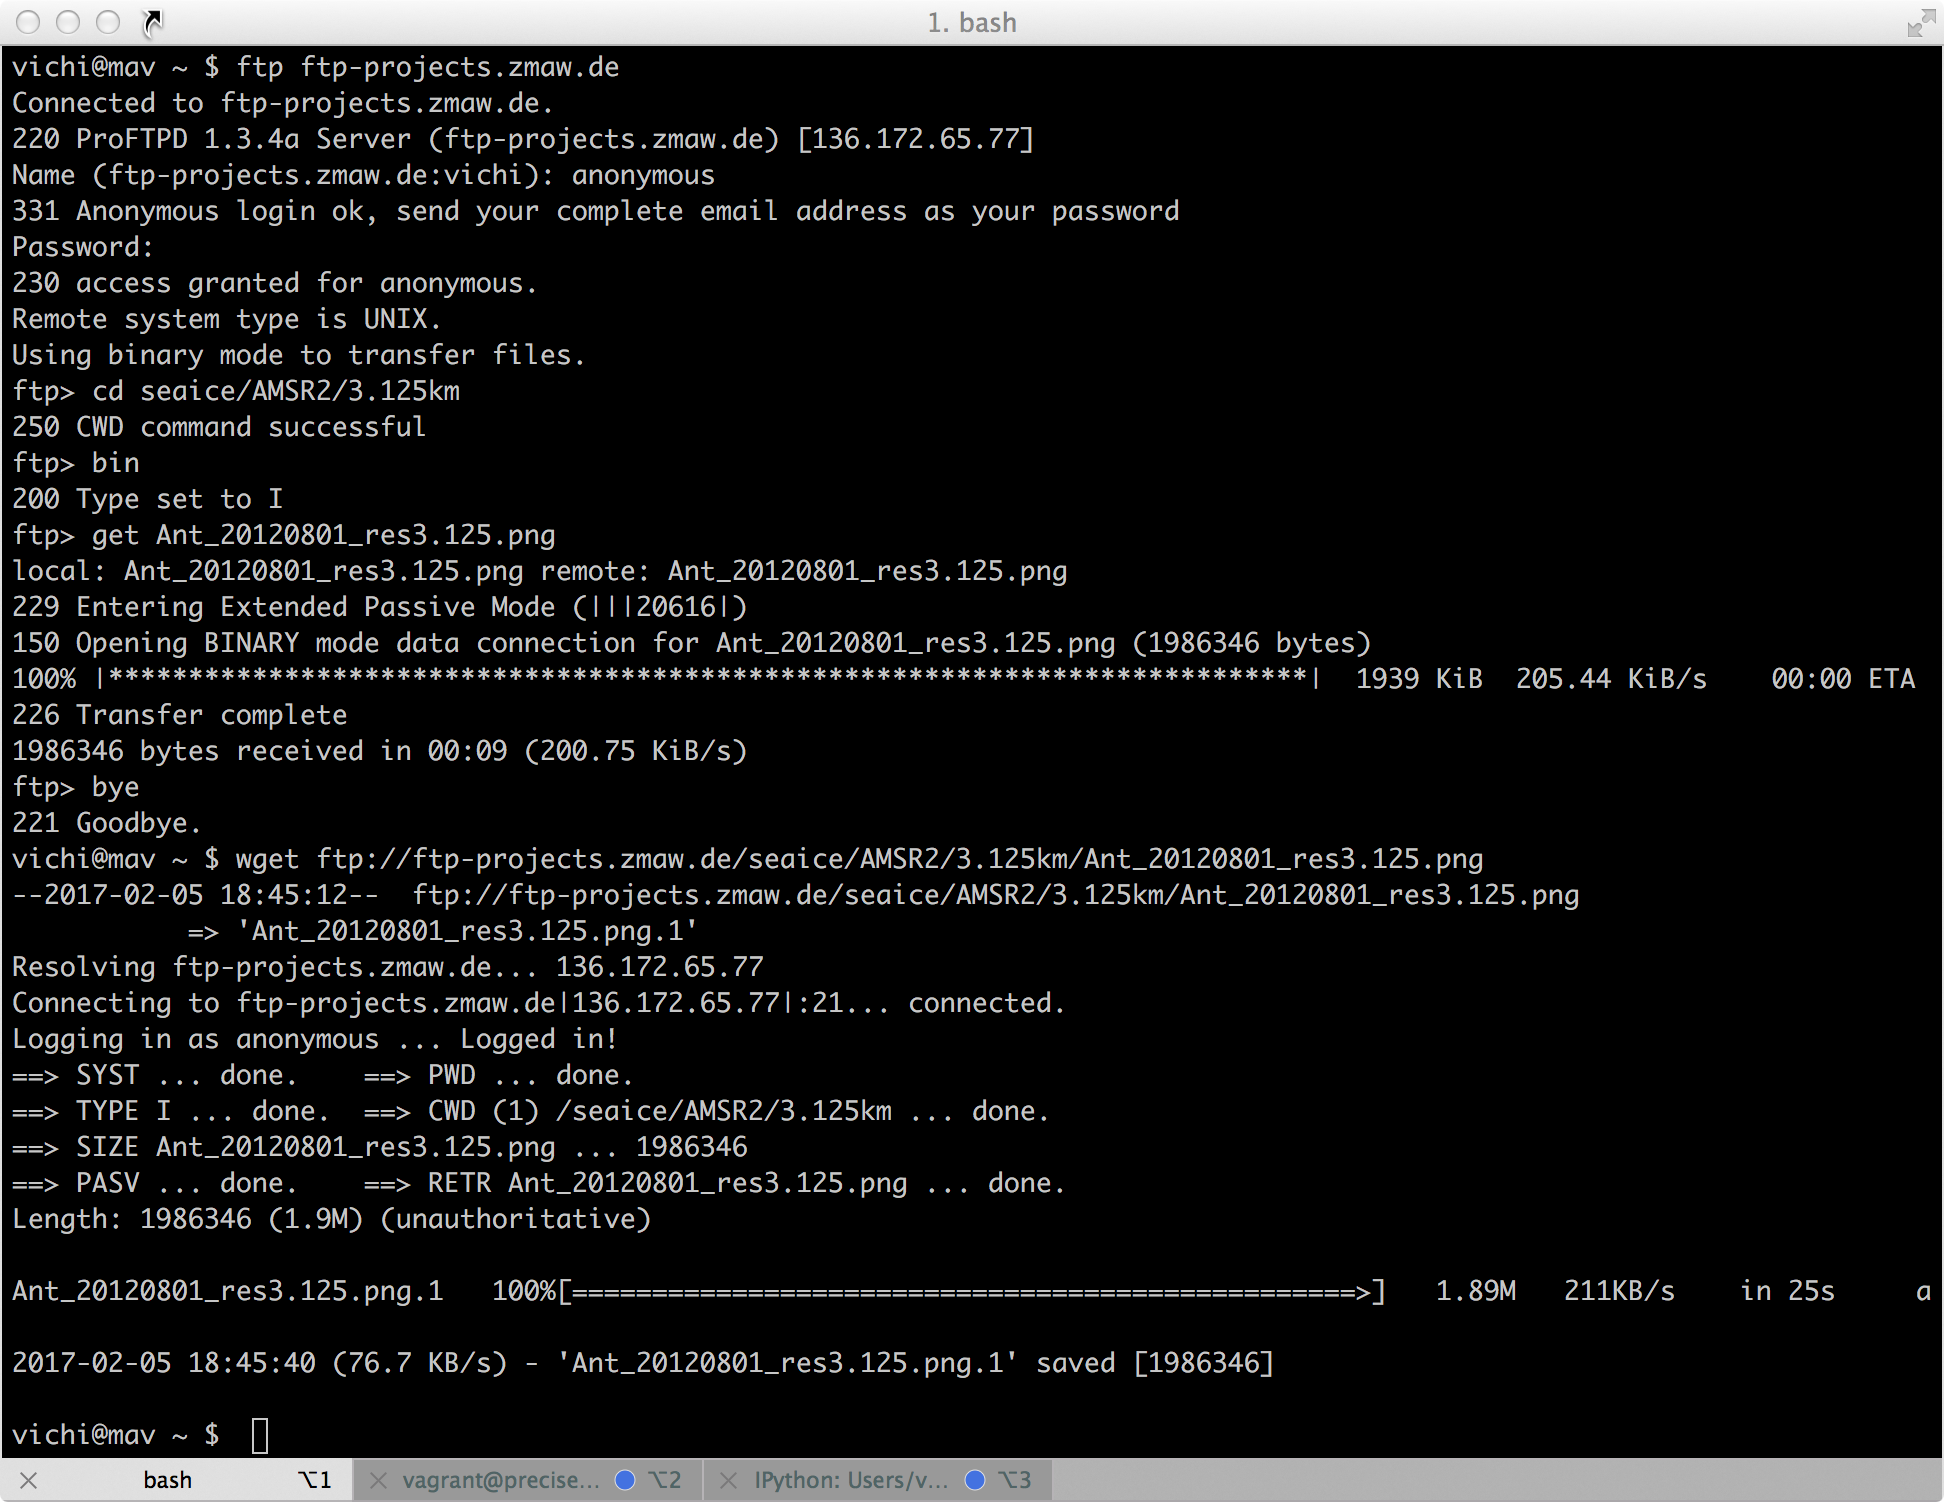
\includegraphics[width=8cm]{figures/ftp-command}
\end{columns}

\end{frame}
%
\begin{frame}{Issues with multiple data transfer}
\begin{columns}[t]

\column{6cm}

\includegraphics[width=6cm]{figures/oceancolor\lyxdot gsfc\lyxdot nasa\lyxdot gov}

\url{https://oceancolor.gsfc.nasa.gov}

\column{6cm}

\includegraphics[width=6cm]{figures/oceancolour\lyxdot org}

\url{https://oceancolour.org}
\end{columns}

\end{frame}
%
\begin{frame}{Giving instructions to the OS: the shell}

Commercial software is not sufficient to perform all the multiple
processing operations needed in ocean sciences. We often have to 
\begin{itemize}
\item download multiple data from different repositories (often at specific
time intervals, e.g. every day)
\item perform the same operation on different files (temporal and spatial
averages, extractions, etc.)
\item rename, cut, concatenate files and convert between different formats
\end{itemize}
All these operations require more than a GUI. This is where the shell
(the language of the terminal) becomes relevant because allows you
to run batch operations (\emph{multiple commands that can be sequentially
executed by the computer, often in the background}). Your computer,
if not a unix OS, is not naturally based on a shell environment. You
then need to prep it and install the proper tools as explained on
the instructions online.
\end{frame}
%
\begin{frame}{Scripting and programming:\ the key to success}

\begin{columns}[t]

\column{6cm}

{\footnotesize{}\url{http://www.nature.com/naturejobs/science/articles/10.1038/nj7638-563a?WT.mc_id=FBK_NatureNews}}{\footnotesize\par}

{\footnotesize{}There are basically 3 choices to combine the computational
capabilities of modern programming languages with processing and analysis
of multidisciplinary ocean data}{\footnotesize\par}
\begin{itemize}
\item \emph{\footnotesize{}Matlab}{\footnotesize{} (commercial software,
open-source version }\emph{\footnotesize{}octave}{\footnotesize{})}{\footnotesize\par}
\item \emph{\footnotesize{}R}{\footnotesize{} (open source)}{\footnotesize\par}
\item \emph{\footnotesize{}Python}{\footnotesize{} (open source)}{\footnotesize\par}
\end{itemize}
{\footnotesize{}They all have pros and cons and they are all interpreted
scripting languages (very high level programming languages; more in
the next lectures). They allow to handle the typical objects of earth
scientists and georeferenced data}{\footnotesize\par}

\column{6cm}
\begin{itemize}
\item {\footnotesize{}Python is the language of choice in this course, but
we will also learn a few shell scripting commands to manipulate files}{\footnotesize\par}
\item {\footnotesize{}Self-learning environment to guide you through the
first steps with python}{\footnotesize\par}
\item {\footnotesize{}on-line assignments will contribute to the final mark
of the module }{\footnotesize\par}
\end{itemize}
\end{columns}

\end{frame}

\end{document}
